\documentclass[11pt]{article}
%\addbibresource{references.bib}

% custom code
\usepackage{xcolor}
\definecolor{light-gray}{gray}{0.75}
\newcommand{\code}[1]{\colorbox{light-gray}{\texttt{#1}}}

% images
\usepackage{graphicx}
\graphicspath{ {./img/} }

% background
\pagecolor{white}


\title{Flatland}
\author{Ryan Kepler Murphy}
\date{\today}

\begin{document}

% Title page
\maketitle	
\pagebreak

% Table of contents
\tableofcontents
\pagebreak

% Paper content

% Problem background
\section{Introduction}
\subsection{Problem Background}
The Flatland framework seeks to address the problem of automated train scheduling and rescheduling, a major challenge
for modern railway systems. It does so by providing a simplified two-dimensional grid world environment to allow for fast experimentation of new approaches to this problem \cite{monylascscbhwaegeibavistsasp20a}. 

\subsection{Related Works}
Scenarios in Flatland exist at the intersection of several well-explored problems.  At its core, Flatland is a multi-agent pathfinding problem; several agents cooperate to complete their goals while managing limited resources within a shared, finite environment.  Outside of pathfinding, Flatland is, in essence, a vehicle rescheduling problem—derived from the vehicle scheduling problem.  An understanding of how each of these problems influences Flatland is a critical piece of finding ideal methods of producing solutions.

\subsubsection{Multi-agent Pathfinding}
Multi-agent pathfinding (MAPF) is a planning problem in which agents in a shared environment must find routes to their respective destinations without incurring collisions \cite{silver05a}.  MAPF has many applications, including in robotics, aviation, and vehicle routing \cite{standley10a}.  Many of the conflicts imposed on agents in MAPF problems are also imposed on agents within the Flatland framework, such as that they may not occupy the same cell at the same time step, or that two agents may not swap positions.  These are to model collisions that would occur in real life.  

Traditional grid environments seen in many MAPF problems, including in \cite{standley10a}, have cells that are often four- or eight-connected; this means that an agent occupying one cell may move to any of its existing unoccupied neighboring cells.  The Flatland framework is more restrictive in this sense, as agents are not free to move to any unoccupied neighboring cell, but rather may move to neighboring cells according to transitions governed by the track type of that cell and the orientation of the agent at that time step, all of which is further discussed in Section \ref{sec:Environment} and can be seen more clearly in Figure \ref{fig:grids}.

% Figure: Grids, degrees of freedom
\begin{figure}[t]
\label{fig:grids}
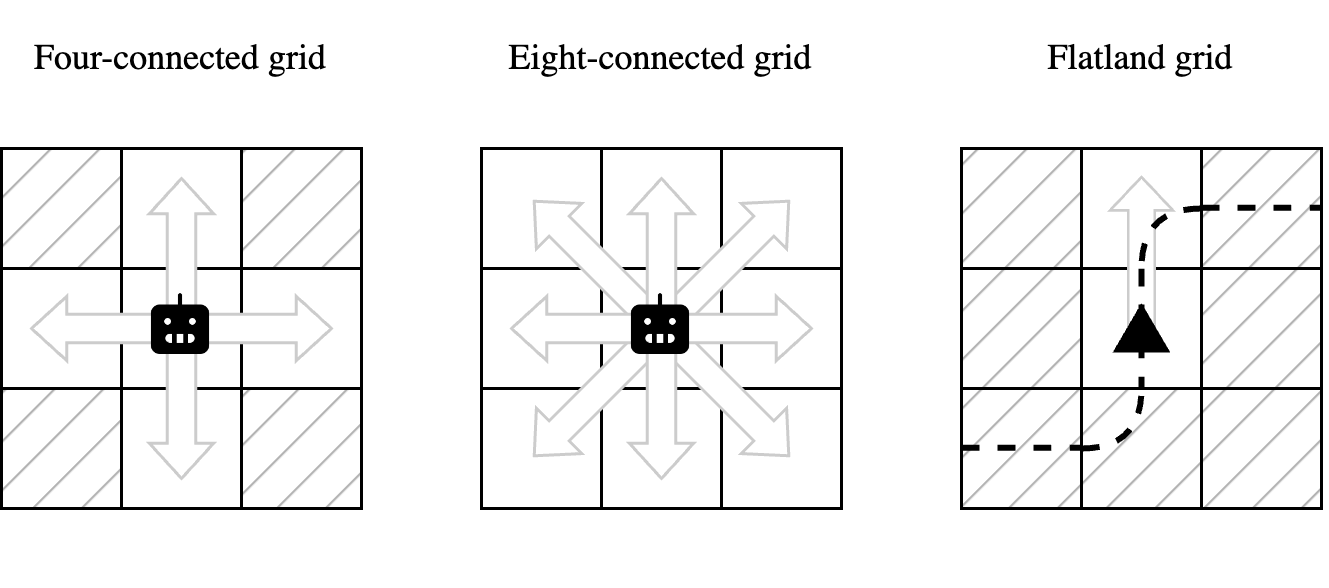
\includegraphics[width=\textwidth]{grids}
\caption{Examples of the degrees of freedom for agents in four-connected grid environments, eight-connected grid environments, and Flatland environments.}
\centering
\end{figure}

\subsubsection{Vehicle Scheduling Problem}
The vehicle scheduling problem (VSP) is a classical optimization problem in the field of operational planning of public transportation systems, consisting of assigning vehicles to trips, in such a way that each trip is associated to one vehicle and a cost function is minimized \cite{bapeukfa00a}.  This problem has been a topic of operational research for decades, but is not the primary focus of Flatland, as each instance already provides a set of agents with pairs of starting and ending positions. Since the agents come pre-assigned to the origin and destination, the importance is shifted from assigning vehicles to trips to actively determining their paths.  However, since Flatland randomly inflicts breakdowns upon its fleet, the task effectively transforms into a vehicle rescheduling problem.

\subsubsection{Vehicle Rescheduling Problem}
The vehicle rescheduling problem (VRSP) is an extension of the VSP and arises when a previously-scheduled trip is disrupted due to interruptions such as a medical emergency or a vehicle breakdown \cite{limibo07a}.  Trips in the Flatland environment model this scenario by randomly assigning vehicle breakdowns, each of which stops a train in its current location for an unforeseen duration.  Ideally, scheduled trips that are affected by a breakdown should be rescheduled in such a way that there are minimal impacts to the original plan.  \cite{limibo07a} note the severity of this problem, in that it results not only in direct operational and delay costs for transit providers, but also in inconvenience for passengers.  The lack of automated rescheduling policies, as well as algorithms that address this problem, highlights the importance of the role that Flatland plays in focusing its scenarios on the element of rescheduling disrupted trips.


% Potential approaches
\section{Approaches}
AIcrowd hosts a global competition in which participants submit crafted approaches to scenarios in the Flatland environment, which are scored and compared against one another.  The variety of submissions highlights the diverse nature of approaches taken to solve the problem Flatland presents.
\subsection{Reinforcement Learning}
There is a separate leaderboard and scoring section for this.

\subsection{Deep Learning}
This was also the focus of some participants.

\subsection{Answer Set Programming}
How is this suitable for this sort of problem?


% The problem workflow
\section{Building Blocks}
Flatland comprises a set of components that are fundamental to its ability to simulate real-world railway scenarios.  In the forefront are the environment and the agents, which form the basis of modeling how trains traverse a physical network.

Further components include the scope of observation, the presence of breakdowns, and pre-determined timetables.  However, these are not considered within the scope of this research.

\subsection{Environment}
\label{sec:Environment}
An environment in Flatland is a grid that consists of cells that are either empty or contain tracks.  A track may belong to one of nine types, and may be rotated in increments of 90º.  Cells must be arranged in such a way that they form a cohesive network, even if the resulting network is simplistic.  Each cell may only be occupied by a single agent at any given time step.  [Transitions are symmetrical]

\subsubsection{Track Types and Transitions}
\label{sec:Track}
Flatland documentation considers seven track types, however, two of them have alternative representations that this paper recognizes as individual types, bringing the total to nine.  There is also a separate designation for an empty cell.

The various rail types can be grouped into two categories: non-switches and switches.  Non-switches include tracks such as straight tracks, curved tracks, and dead ends.  [They do not allow the course of the path to change.]  Conversely, switches represent a decision point, as they force agents to make a choice.  A switch will never present more than two options.

Each rail type determines the possible transitions for the agents, meaning which neighboring cells are accessible positions following a single move.  Crucially, neighboring cells that are accessible from one location, may in some cases not be accessible had the train approached this same location from another direction.  For this reason, recording both the position and orientation of each agents at every time step is necessary for determining its legal paths.  A diagram explaining this quality is shown in Figure \ref{fig:transitions}.

\subsubsection{Points of Interest}
[Stations and cities]


\subsection{Agents}
\label{sec:Agents}
Agents in Flatland represent the trains of a railway network.  They can choose from a set of actions, are given starting locations and specified destinations, must avoid collisions and other conflicts with agents present throughout the environment, and have various speed profiles.  The terms \textit{agent} and \textit{train} are used interchangeably.

\subsubsection{Actions}
\label{sec:Actions}
Within the environment, agents follow a series of actions.  Since Flatland is a discrete time simulation, the duration of each action conforms to a constant amount of time.    At each time step, agents must choose from one of the following five actions: 
\begin{enumerate}
  \item \code{MOVE\_FORWARD}: this action moves the train forward, provided there is a legal transition that allows this; this is also the appropriate action along curved track with no switch
  \item \code{MOVE\_LEFT}: this action moves the train along a switch to the left, provided there is a legal transition that allows this
  \item \code{MOVE\_RIGHT}: this action moves the train along a switch to the right, provided there is a legal transition that allows this
  \item \code{STOP\_MOVING}: this action stops the train, resulting in its remaining in the current cell
  \item\code{{DO\_NOTHING}}: this action compels the train to adhere to a continuation of its previous action; the one exception is that while stopped in a dead end, this reverses the direction of the train
\end{enumerate} \smallskip

\noindent So long as a valid action has been selected, the position and orientation of the agent will be updated in the following time step. \medskip

\subsubsection{Starting and Ending Positions}
\label{sec:Positions}
Each agent is given a starting position and orientation, as well as a destination.  The goal for a single agent is to traverse the environment by choosing valid actions along legal paths that lead the agent from its starting position to its destination.  

For simplicity, trains are not recognized by the environment until they are actively underway.  This prevents trains who have not yet begun their journeys from occupying space on the tracks and preventing the passage of other trains.  Likewise, once a train reaches its destination, it is no longer recognized as actively being present in the environment.  The track space therefore becomes free in the time step after the train has completed its journey.

\subsubsection{Conflicts and Speed Profiles}
\label{sec:Conflicts}
Consistent with core tenets of any MAPF problem, any two trains must avoid a collision with each other.  Agents, as with trains in real life, may not physically pass through one another.  This prevents one train from overtaking a stopped train on the same set of tracks; it also prevents two trains facing each other from swapping positions.

Furthermore, agents in Flatland may have different speeds, depending on their train types, such as passenger trains or freight trains.  This speed profile determines how quickly agents are capable of traversing the environment, and ultimately influences how they interact with one another.  [This means] that a train cannot travel faster than another train traveling immediately before it.



\bibliographystyle{plain}
\bibliography{references}
\end{document}